\section{IoTサービス}
% (IoTサービスがどのようなもので,どのような背景で登場してきたのか,どんなものがありどのような自動化を図っているのか)}
IoTとは,Internet of Things の略で「モノのインターネット」とも呼ばれる概念である.
IoTでは,様々な物がインターネットにつながり,相互に情報をやり取りすることで,多様な自動化を行う.
IoTサービスとは,ユーザーに対しIoTによる利便性を提供するものである.
\medskip

IoTサービスは,半導体技術の進歩によりコンピューターが小型且つ安価になったこと,通信ネットワークの整備が進み様々な場所から安価に通信が利用可能になったことで登場した.
\medskip

例えば,次のような物がある.
\begin{itemize}
	\item 駐車場の検索・予約・決済サービス\cite{エコパ}
	\item 太陽光発電の監視
\end{itemize}

駐車場の検索・予約・決済サービスとは,ドライバーが空いている駐車場を探す手間を省くためのサービスである.
周囲の空いている駐車場の検索や,予め駐車場を予約しておくことで,駐車場を探す手間を省いている.
このサービスの実現のために,駐車場の駐車スペースにコンピュータを取り付ける.
これらコンピュータが,駐車場が空いているか否か・予約が入っているか否か等をサーバーとやり取りする.
それらにより,サーバーは空いている駐車場の一覧や,利用情報に基づく決済を,ユーザーに提供している.
\medskip

太陽光発電の監視とは,太陽光発電所の発電量や機器の異常を確認しに行くための手間を省くためのサービスである.
このサービスの実現の為に,太陽光発電所の機器にコンピューターを取り付ける.
これらコンピュータが発電量や機器の異常の情報をサーバーとやり取りする.
それにより,サーバーは,発電量や機器の異常をユーザーに知らせる.
\medskip

このように,IoTサービスは,IoT機器とサーバーが連携し,ユーザーに利便性を提供するものである.
今後も数多くサービスが登場すると考えられている.

\section{IoTサービスの構造}
%(IoTサービスの構造要素としてIoT機器とサーバがあること,IoT機器・サーバーとはどのようなものなのか,何をしているのか,その間の通信とはどのようなものなのか)
IoTサービスは,IoT機器とサーバーが連携し利便性を提供するものである.
IoTサービスは,多数のIoT機器とサーバーがインターネットを介し連携する構造になっている。
\medskip

\begin{figure}[htbp]
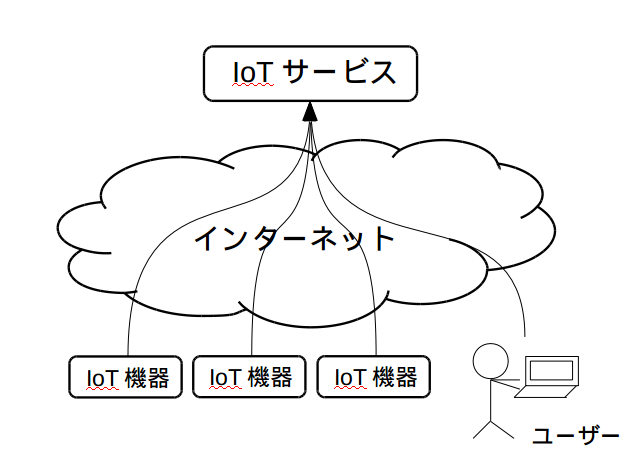
\includegraphics[width=14cm]{images/IoTservice.png}
\caption{IoTサービスの構成図}
\label{fig:IoTservice}
\end{figure}

IoT機器は,様々な環境へ設置され,周囲の状況を検知することや,周囲へなんらかの働きを行う為に使用される.
駐車場の例では,駐車スペースに車が止まっているか否かを検知している.
IoT機器の上では、サーバと情報を送受するプログラムが常時動作し、周囲の状況をサーバーに送信するか、サーバへ周囲へ何らかの働きかけを行うかどうか問い合わせている。
\medskip

この機器からの情報を収集し,処理しているのがサーバーである.
サーバーは,IoT機器からの情報を蓄積・分析し,IoT機器やユーザーに対し何らかの働きかけを行う.
駐車場の例では,駐車場の利用情報を蓄積・分析し,ユーザーへ対し可視化を行っている.
サーバーにて動作するプログラムが,IoT機器と通信することで,IoTサービスを構成する.
この通信に利用されるのがインターネットである.
様々な通信リンクを用いてIoT機器とサーバー上のプログラムが連携する.
\medskip


ユーザーは、サーバが蓄積・分析した情報を閲覧したり、サーバが蓄積・分析した情報をもととした通知を受け取る。

このように,IoTサービスの構造は,IoT機器とサーバー上のプログラムがインターネットを介し通信し,連携することで成り立っている.
図\ref{fig:IoTservice}は,IoTサービスの構造図である


\section{IoTサービスの開発・運用の事例}
IoTサービスの開発・運用における課題を分析するために、実験およびヒアリングを行った。
\subsection{岡本商店街での実験}
\input okamoto.tex

\subsection{株式会社ルナネクサスへの聞き取り}
\input lunanexus.tex

%開発と運用が大変であること言うために、岡本商店街とルナネクサスさんの話をする

\section{IoTサービスの提供者の課題}
%IoTサービスを開発、運用する人達として、開発者と運用者が居ることを紹介する。
IoTサービスは、IoT機器とサーバ上のプログラムがインターネットを介し通信し合うことで成り立っている。
このような構造を持つIoTサービスの提供は、それぞれ異なった役割を持つ開発者と運用者が行っている。
開発者はサービスを設計・構築し、運用者はサービスによる供給が止まらないように維持・管理する役割を持っている。

%IoTサービス開発にはどのような問題があるのか説明する。
%IoTサービス開発の何がどう大変なのか、開発者の視点で説明する。
IoTサービスの開発には、次のような問題がある。
\begin{itemize}
\item 多分野に渡る技術を知っていなければならない\\
	IoT機器の開発には、ハードウェアの知識や、ネットワークの知識が必要不可欠である。
	また、サービスプログラム(?)の開発のためには、データベースやネットワークの知識が必要となる。
	このように、多分野に渡る知識を知っていなければ、開発することができない。
\item 一つの機能を実装するだけでも困難な作業である\\
	IoTサービスは、一つの機能を別々の機器上で動く複数のプログラム間のやり取りにて実現するため、簡単な機能であっても、すぐに実現可能なわけではない。
\item 設置やトラブル対応が難しい\\
	IoTサービスの開発には、多分野に渡る技術を知っていなければならないため、
	トラブルが発生した場合、知識のある開発者が現地に行かなければならず、コストが高い。
	また、設置の時も同様で、予め開発者が現地に行き設置環境を確認しなければならない。
\item ネットワークの監視はIoTサービスが提供する機能とは別の機能である\\
	ネットワークの監視やIoT機器の監視は、IoTサービスが提供する機能とは別の機能である。
	そのため、IoTサービスをもうひとつ作るのと変わらない手間がかかり、開発者の負担となっている。
\end{itemize}
このように、IoTサービスの開発は、開発者の負担が大きい。

%IoTサービスの運用にはどのような問題があるのか説明する。
%IoTサービスの運用者はどう大変なのか、説明する。(IoTサービスの構造を維持することが大変という)
また、IoTサービスの維持・管理においては、次のような課題がある。
\begin{itemize}
\item IoT機器の接続されるネットワークは想定できない\\
	IoT機器が接続されるネットワークは、IoT機器の移動や既設ネットワークへの接続の事を考えると、予め想定することが難しい。
	そのため、サーバに対し、予め設置することは困難である。
\item IoT機器の接続されるネットワークがプライベートアドレスであることがある\\
	IoT機器の接続されるネットワークは、利便性の都合などからプライベートアドレスを利用し、インターネットとの接続点にNAPTが置かれる事がある。
	そのため、サーバからの通信が遮断されることがある。
\item IoT機器は安価なため、大量に利用される\\
	IoT機器は安価であるため、大量に利用されることが多い。
	そのため、サーバー側へ設定することは負担が大きい。?
\end{itemize}
このような問題から、IoTサービスの開発・運用は開発者や運用者の負担となっている。



\section{考察}
%IoTサービスの構造の維持が必要で、維持の為に、監視が必要となっている
%また、その監視は注ぎのヨ兼を満たしている必要がある。
\begin{comment}
この考察の中で、「開発者」の視点を入れて説明してください。
誰がどのように困っているのかをはっきり説明して、そのうえでどうあるべきかの要件の説明です。
「運用者」の視点も混ざると大変だと思うので、ひとまず「開発者」=「運用者」というつもりで書いてくれていいです。
IoTサービスの開発運用の困難ということで。
\end{comment}
このように、開発者・運用者は、構造の複雑さ・利便性から困っている。
ここから、私は、次のような点を問題として取り上げた。
\begin{itemize}
\item IoT機器の監視は必要だが、技術的な問題により、既存の監視手法では監視しづらい
%\\	株式会社ルナネクサスの事例でも、岡本商店街の事例でも、IoT機器が接続されるネットワークが様々である(になる予定である)ことから、監視が難しくなっている。
\item IoT機器の監視問題の解決の為に、開発者の負担が大きくなっている
%\\	2事例にて、機器の監視の解決の為に、開発者の負担が大きくなっていることが分かった。
\end{itemize}


また、これら実験やヒアリングの結果から、監視には次のような物が求められていることが分かった。
\begin{itemize}
\item IoT機器の接続されるネットワークが、プライベートアドレスを使用していても、監視可能であること\\
	IoT機器が接続されるネットワークを予め予測することは難しい。
	そのため、IoT機器にプライベートアドレスが割り振られる可能性がある。
	そのような状況でも監視することができる必要がある。
\item ネットワークが違っていても、一つの画面で確認できること\\
\item IoTサービスの変更が不要であること\\
	サーバの変更は開発者への負担となるため、サーバの変更を避けたい。
\item 監視サーバを立てる必要がないこと\\
	新たに監視サーバを立てることは、設定や構築作業が必要となるため、開発者の負担となる。
	そのため、新規に監視サーバを立てる必要が無いことが求められる。
\end{itemize}



\begin{comment}
具体的には次のような技術的困難がある。
\begin{itemize}
\item IoT機器が設置されるネットワーク環境が様々\\
	\begin{itemize}
		\item IoT機器が設置されるネットワークが、NAPTの下にある場合がある。\\
			NAPTとは、Network Address Port Transraterの事で、内側のネットワークのみで通用するIPアドレスとポート番号を必要に応じて、インターネット上で通用するIPアドレスとポート番号に変換する。
			変換の際、一時的にIPアドレスとポート番号の組み合わせを記憶し、返信があった際、記憶していたIPアドレスとポート番号の組み合わせを用いて内側のネットワークに転送する。
			そのため、内側から始まる通信は問題ないが、インターネット側から始まる通信はブロックされる。
			よって、機器監視サーバからIoT機器に対して状態を問い合わせることが出来ない。
			また、NAPT下に複数の機器が存在する場合、IPアドレスにて機器の識別をしていると、機器監視サービス側からは同一のIPアドレスからの通信に見えるので、機器が判別出来ない問題がある。
		\item IoT機器が移動する物だと、ネットワークが切り替わる場合がある。\\
			IoT機器が移動する機器である場合、ネットワークが切り替わる場合がある。
			例えば、家の中では、家に敷設されたインターネット回線を用いてインターネットへ出るが、外出先では携帯電話網を利用しているといった事があげられる。
			IPアドレスにて機器の識別をしている場合、別の機器からの通信のようにみえてしまう。
		\item セキュリティの都合上、ブロックされている場合がある。\\
			SNMPやPing等、攻撃の足がかりとなりうるプロトコルについて、ブロックされている場合がある。
			IoT機器が設置される環境によっては、機器の通信の為にブロックを解除するなどの手間が発生するが、設置される機器のネットワークが借り物である場合などは、難しい。
	\end{itemize}
\item 多量のIoT機器が存在する
	\begin{itemize}
		\item 機器監視サービスによっては、機器を追加する毎に繁雑な手順を踏まなくてはならない。
	\end{itemize}
\end{itemize}
IoTサービスの管理者が監視をしているが、監視に係る手間や監視の為に必要なことが多く困っている事を言いたい。
\end{comment}

